\documentclass[1p]{elsarticle_modified}
%\bibliographystyle{elsarticle-num}

%\usepackage[colorlinks]{hyperref}
%\usepackage{abbrmath_seonhwa} %\Abb, \Ascr, \Acal ,\Abf, \Afrak
\usepackage{amsfonts}
\usepackage{amssymb}
\usepackage{amsmath}
\usepackage{amsthm}
\usepackage{scalefnt}
\usepackage{amsbsy}
\usepackage{kotex}
\usepackage{caption}
\usepackage{subfig}
\usepackage{color}
\usepackage{graphicx}
\usepackage{xcolor} %% white, black, red, green, blue, cyan, magenta, yellow
\usepackage{float}
\usepackage{setspace}
\usepackage{hyperref}

\usepackage{tikz}
\usetikzlibrary{arrows}

\usepackage{multirow}
\usepackage{array} % fixed length table
\usepackage{hhline}

%%%%%%%%%%%%%%%%%%%%%
\makeatletter
\renewcommand*\env@matrix[1][\arraystretch]{%
	\edef\arraystretch{#1}%
	\hskip -\arraycolsep
	\let\@ifnextchar\new@ifnextchar
	\array{*\c@MaxMatrixCols c}}
\makeatother %https://tex.stackexchange.com/questions/14071/how-can-i-increase-the-line-spacing-in-a-matrix
%%%%%%%%%%%%%%%

\usepackage[normalem]{ulem}

\newcommand{\msout}[1]{\ifmmode\text{\sout{\ensuremath{#1}}}\else\sout{#1}\fi}
%SOURCE: \msout is \stkout macro in https://tex.stackexchange.com/questions/20609/strikeout-in-math-mode

\newcommand{\cancel}[1]{
	\ifmmode
	{\color{red}\msout{#1}}
	\else
	{\color{red}\sout{#1}}
	\fi
}

\newcommand{\add}[1]{
	{\color{blue}\uwave{#1}}
}

\newcommand{\replace}[2]{
	\ifmmode
	{\color{red}\msout{#1}}{\color{blue}\uwave{#2}}
	\else
	{\color{red}\sout{#1}}{\color{blue}\uwave{#2}}
	\fi
}

\newcommand{\Sol}{\mathcal{S}} %segment
\newcommand{\D}{D} %diagram
\newcommand{\A}{\mathcal{A}} %arc


%%%%%%%%%%%%%%%%%%%%%%%%%%%%%5 test

\def\sl{\operatorname{\textup{SL}}(2,\Cbb)}
\def\psl{\operatorname{\textup{PSL}}(2,\Cbb)}
\def\quan{\mkern 1mu \triangleright \mkern 1mu}

\theoremstyle{definition}
\newtheorem{thm}{Theorem}[section]
\newtheorem{prop}[thm]{Proposition}
\newtheorem{lem}[thm]{Lemma}
\newtheorem{ques}[thm]{Question}
\newtheorem{cor}[thm]{Corollary}
\newtheorem{defn}[thm]{Definition}
\newtheorem{exam}[thm]{Example}
\newtheorem{rmk}[thm]{Remark}
\newtheorem{alg}[thm]{Algorithm}

\newcommand{\I}{\sqrt{-1}}
\begin{document}

%\begin{frontmatter}
%
%\title{Boundary parabolic representations of knots up to 8 crossings}
%
%%% Group authors per affiliation:
%\author{Yunhi Cho} 
%\address{Department of Mathematics, University of Seoul, Seoul, Korea}
%\ead{yhcho@uos.ac.kr}
%
%
%\author{Seonhwa Kim} %\fnref{s_kim}}
%\address{Center for Geometry and Physics, Institute for Basic Science, Pohang, 37673, Korea}
%\ead{ryeona17@ibs.re.kr}
%
%\author{Hyuk Kim}
%\address{Department of Mathematical Sciences, Seoul National University, Seoul 08826, Korea}
%\ead{hyukkim@snu.ac.kr}
%
%\author{Seokbeom Yoon}
%\address{Department of Mathematical Sciences, Seoul National University, Seoul, 08826,  Korea}
%\ead{sbyoon15@snu.ac.kr}
%
%\begin{abstract}
%We find all boundary parabolic representation of knots up to 8 crossings.
%
%\end{abstract}
%\begin{keyword}
%    \MSC[2010] 57M25 
%\end{keyword}
%
%\end{frontmatter}

%\linenumbers
%\tableofcontents
%
\newcommand\colored[1]{\textcolor{white}{\rule[-0.35ex]{0.8em}{1.4ex}}\kern-0.8em\color{red} #1}%
%\newcommand\colored[1]{\textcolor{white}{ #1}\kern-2.17ex	\textcolor{white}{ #1}\kern-1.81ex	\textcolor{white}{ #1}\kern-2.15ex\color{red}#1	}

{\Large $\underline{12a_{0872}~(K12a_{0872})}$}

\setlength{\tabcolsep}{10pt}
\renewcommand{\arraystretch}{1.6}
\vspace{1cm}\begin{tabular}{m{100pt}>{\centering\arraybackslash}m{274pt}}
\multirow{5}{120pt}{
	\centering
	\includegraphics[width=112pt]{../../../GIT/diagram.site/Diagrams/png/1673_12a_0872.png}\\
\ \ \ A knot diagram\footnotemark}&
\allowdisplaybreaks
\textbf{Linearized knot diagam} \\
\cline{2-2}
 &
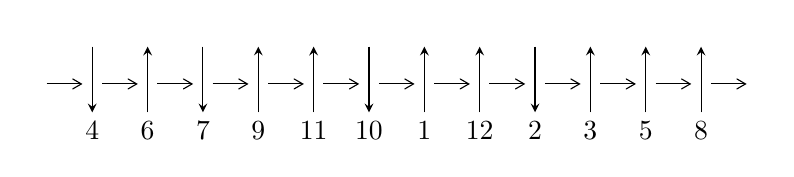
\begin{tikzpicture}[x=20pt, y=17pt]
	% nodes
	\node (C0) at (0, 0) {};
	\node (C1) at (1, 0) {};
	\node (C1U) at (1, +1) {};
	\node (C1D) at (1, -1) {4};

	\node (C2) at (2, 0) {};
	\node (C2U) at (2, +1) {};
	\node (C2D) at (2, -1) {6};

	\node (C3) at (3, 0) {};
	\node (C3U) at (3, +1) {};
	\node (C3D) at (3, -1) {7};

	\node (C4) at (4, 0) {};
	\node (C4U) at (4, +1) {};
	\node (C4D) at (4, -1) {9};

	\node (C5) at (5, 0) {};
	\node (C5U) at (5, +1) {};
	\node (C5D) at (5, -1) {11};

	\node (C6) at (6, 0) {};
	\node (C6U) at (6, +1) {};
	\node (C6D) at (6, -1) {10};

	\node (C7) at (7, 0) {};
	\node (C7U) at (7, +1) {};
	\node (C7D) at (7, -1) {1};

	\node (C8) at (8, 0) {};
	\node (C8U) at (8, +1) {};
	\node (C8D) at (8, -1) {12};

	\node (C9) at (9, 0) {};
	\node (C9U) at (9, +1) {};
	\node (C9D) at (9, -1) {2};

	\node (C10) at (10, 0) {};
	\node (C10U) at (10, +1) {};
	\node (C10D) at (10, -1) {3};

	\node (C11) at (11, 0) {};
	\node (C11U) at (11, +1) {};
	\node (C11D) at (11, -1) {5};

	\node (C12) at (12, 0) {};
	\node (C12U) at (12, +1) {};
	\node (C12D) at (12, -1) {8};
	\node (C13) at (13, 0) {};

	% arrows
	\draw[->,>={angle 60}]
	(C0) edge (C1) (C1) edge (C2) (C2) edge (C3) (C3) edge (C4) (C4) edge (C5) (C5) edge (C6) (C6) edge (C7) (C7) edge (C8) (C8) edge (C9) (C9) edge (C10) (C10) edge (C11) (C11) edge (C12) (C12) edge (C13) ;	\draw[->,>=stealth]
	(C1U) edge (C1D) (C2D) edge (C2U) (C3U) edge (C3D) (C4D) edge (C4U) (C5D) edge (C5U) (C6U) edge (C6D) (C7D) edge (C7U) (C8D) edge (C8U) (C9U) edge (C9D) (C10D) edge (C10U) (C11D) edge (C11U) (C12D) edge (C12U) ;
	\end{tikzpicture} \\
\hhline{~~} \\& 
\textbf{Solving Sequence} \\ \cline{2-2} 
 &
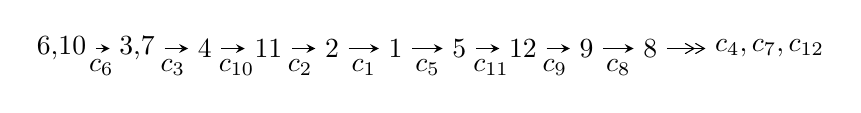
\begin{tikzpicture}[x=23pt, y=7pt]
	% node
	\node (A0) at (-1/8, 0) {6,10};
	\node (A1) at (17/16, 0) {3,7};
	\node (A2) at (17/8, 0) {4};
	\node (A3) at (25/8, 0) {11};
	\node (A4) at (33/8, 0) {2};
	\node (A5) at (41/8, 0) {1};
	\node (A6) at (49/8, 0) {5};
	\node (A7) at (57/8, 0) {12};
	\node (A8) at (65/8, 0) {9};
	\node (A9) at (73/8, 0) {8};
	\node (C1) at (1/2, -1) {$c_{6}$};
	\node (C2) at (13/8, -1) {$c_{3}$};
	\node (C3) at (21/8, -1) {$c_{10}$};
	\node (C4) at (29/8, -1) {$c_{2}$};
	\node (C5) at (37/8, -1) {$c_{1}$};
	\node (C6) at (45/8, -1) {$c_{5}$};
	\node (C7) at (53/8, -1) {$c_{11}$};
	\node (C8) at (61/8, -1) {$c_{9}$};
	\node (C9) at (69/8, -1) {$c_{8}$};
	\node (A10) at (11, 0) {$c_{4},c_{7},c_{12}$};

	% edge
	\draw[->,>=stealth]	
	(A0) edge (A1) (A1) edge (A2) (A2) edge (A3) (A3) edge (A4) (A4) edge (A5) (A5) edge (A6) (A6) edge (A7) (A7) edge (A8) (A8) edge (A9) ;
	\draw[->>,>={angle 60}]	
	(A9) edge (A10);
\end{tikzpicture} \\ 

\end{tabular} \\

\footnotetext{
The image of knot diagram is generated by the software ``\textbf{Draw programme}" developed by Andrew Bartholomew(\url{http://www.layer8.co.uk/maths/draw/index.htm\#Running-draw}), where we modified some parts for our purpose(\url{https://github.com/CATsTAILs/LinksPainter}).
}\phantom \\ \newline 
\centering \textbf{Ideals for irreducible components\footnotemark of $X_{\text{par}}$} 
 
\begin{align*}
I^u_{1}&=\langle 
1.30286\times10^{835} u^{127}+6.91127\times10^{835} u^{126}+\cdots+1.24523\times10^{836} b+3.82455\times10^{835},\\
\phantom{I^u_{1}}&\phantom{= \langle  }-2.22805\times10^{837} u^{127}-3.94170\times10^{837} u^{126}+\cdots+1.24523\times10^{836} a+1.79835\times10^{836},\\
\phantom{I^u_{1}}&\phantom{= \langle  }5 u^{128}+6 u^{127}+\cdots+3 u-1\rangle \\
I^u_{2}&=\langle 
-2.14762\times10^{46} u^{29}-1.35976\times10^{47} u^{28}+\cdots+8.51286\times10^{45} b-1.05226\times10^{46},\\
\phantom{I^u_{2}}&\phantom{= \langle  }3.44982\times10^{46} u^{29}+2.00343\times10^{47} u^{28}+\cdots+8.51286\times10^{45} a+1.52741\times10^{46},\;5 u^{30}+33 u^{29}+\cdots+2 u+1\rangle \\
\\
\end{align*}
\raggedright * 2 irreducible components of $\dim_{\mathbb{C}}=0$, with total 158 representations.\\
\footnotetext{All coefficients of polynomials are rational numbers. But the coefficients are sometimes approximated in decimal forms when there is not enough margin.}
\newpage
\renewcommand{\arraystretch}{1}
\centering \section*{I. $I^u_{1}= \langle 1.30\times10^{835} u^{127}+6.91\times10^{835} u^{126}+\cdots+1.25\times10^{836} b+3.82\times10^{835},\;-2.23\times10^{837} u^{127}-3.94\times10^{837} u^{126}+\cdots+1.25\times10^{836} a+1.80\times10^{836},\;5 u^{128}+6 u^{127}+\cdots+3 u-1 \rangle$}
\flushleft \textbf{(i) Arc colorings}\\
\begin{tabular}{m{7pt} m{180pt} m{7pt} m{180pt} }
\flushright $a_{6}=$&$\begin{pmatrix}1\\0\end{pmatrix}$ \\
\flushright $a_{10}=$&$\begin{pmatrix}0\\u\end{pmatrix}$ \\
\flushright $a_{3}=$&$\begin{pmatrix}17.8927 u^{127}+31.6544 u^{126}+\cdots-38.4932 u-1.44419\\-0.104628 u^{127}-0.555020 u^{126}+\cdots+3.04440 u-0.307136\end{pmatrix}$ \\
\flushright $a_{7}=$&$\begin{pmatrix}1\\u^2\end{pmatrix}$ \\
\flushright $a_{4}=$&$\begin{pmatrix}23.8766 u^{127}+42.3995 u^{126}+\cdots-44.0690 u+0.899592\\2.07893 u^{127}+3.35288 u^{126}+\cdots+2.10257 u+0.405735\end{pmatrix}$ \\
\flushright $a_{11}=$&$\begin{pmatrix}56.8012 u^{127}+102.085 u^{126}+\cdots+21.2724 u+9.74949\\4.66762 u^{127}+7.89060 u^{126}+\cdots+5.94744 u+1.35955\end{pmatrix}$ \\
\flushright $a_{2}=$&$\begin{pmatrix}17.9973 u^{127}+32.2095 u^{126}+\cdots-41.5376 u-1.13705\\-0.104628 u^{127}-0.555020 u^{126}+\cdots+3.04440 u-0.307136\end{pmatrix}$ \\
\flushright $a_{1}=$&$\begin{pmatrix}-9.39015 u^{127}-13.4013 u^{126}+\cdots-13.6158 u-9.85715\\2.28571 u^{127}+4.94598 u^{126}+\cdots+2.20477 u-0.129018\end{pmatrix}$ \\
\flushright $a_{5}=$&$\begin{pmatrix}-51.8393 u^{127}-102.851 u^{126}+\cdots-104.441 u-18.1579\\-8.81590 u^{127}-16.5949 u^{126}+\cdots+0.826844 u-3.72755\end{pmatrix}$ \\
\flushright $a_{12}=$&$\begin{pmatrix}1.88284 u^{127}+10.1744 u^{126}+\cdots+6.94980 u+3.35617\\4.22223 u^{127}+8.39879 u^{126}+\cdots-7.69204 u+0.894113\end{pmatrix}$ \\
\flushright $a_{9}=$&$\begin{pmatrix}47.4844 u^{127}+86.0915 u^{126}+\cdots+11.9416 u+7.09790\\4.64910 u^{127}+8.10242 u^{126}+\cdots+5.38331 u+1.29204\end{pmatrix}$ \\
\flushright $a_{8}=$&$\begin{pmatrix}-33.4742 u^{127}-65.6211 u^{126}+\cdots+36.3065 u-9.46504\\-12.7668 u^{127}-24.5715 u^{126}+\cdots+11.3679 u-3.58033\end{pmatrix}$\\&\end{tabular}
\flushleft \textbf{(ii) Obstruction class $= -1$}\\~\\
\flushleft \textbf{(iii) Cusp Shapes $= -4.75828 u^{127}-9.80991 u^{126}+\cdots+10.3737 u+5.73316$}\\~\\
\newpage\renewcommand{\arraystretch}{1}
\flushleft \textbf{(iv) u-Polynomials at the component}\newline \\
\begin{tabular}{m{50pt}|m{274pt}}
Crossings & \hspace{64pt}u-Polynomials at each crossing \\
\hline $$\begin{aligned}c_{1}\end{aligned}$$&$\begin{aligned}
&5(5 u^{128}+44 u^{127}+\cdots+774818 u-401483)
\end{aligned}$\\
\hline $$\begin{aligned}c_{2}\end{aligned}$$&$\begin{aligned}
&u^{128}- u^{127}+\cdots+181885 u+12725
\end{aligned}$\\
\hline $$\begin{aligned}c_{3}\end{aligned}$$&$\begin{aligned}
&u^{128}-4 u^{127}+\cdots-11825779033 u+7211692781
\end{aligned}$\\
\hline $$\begin{aligned}c_{4}\end{aligned}$$&$\begin{aligned}
&u^{128}+u^{127}+\cdots+1190911161 u+121993295
\end{aligned}$\\
\hline $$\begin{aligned}c_{5},c_{11}\end{aligned}$$&$\begin{aligned}
&5(5 u^{128}-6 u^{127}+\cdots+40667 u+8021)
\end{aligned}$\\
\hline $$\begin{aligned}c_{6}\end{aligned}$$&$\begin{aligned}
&5(5 u^{128}-6 u^{127}+\cdots-3 u-1)
\end{aligned}$\\
\hline $$\begin{aligned}c_{7},c_{8},c_{12}\end{aligned}$$&$\begin{aligned}
&u^{128}+69 u^{126}+\cdots+3101 u+335
\end{aligned}$\\
\hline $$\begin{aligned}c_{9}\end{aligned}$$&$\begin{aligned}
&u^{128}- u^{127}+\cdots+109650874 u+30512188
\end{aligned}$\\
\hline $$\begin{aligned}c_{10}\end{aligned}$$&$\begin{aligned}
&u^{128}+u^{127}+\cdots-86689 u+15995
\end{aligned}$\\
\hline
\end{tabular}\\~\\
\newpage\renewcommand{\arraystretch}{1}
\flushleft \textbf{(v) Riley Polynomials at the component}\newline \\
\begin{tabular}{m{50pt}|m{274pt}}
Crossings & \hspace{64pt}Riley Polynomials at each crossing \\
\hline $$\begin{aligned}c_{1}\end{aligned}$$&$\begin{aligned}
&25(25 y^{128}-1586 y^{127}+\cdots-2.34182\times10^{13} y+1.61189\times10^{11})
\end{aligned}$\\
\hline $$\begin{aligned}c_{2}\end{aligned}$$&$\begin{aligned}
&y^{128}+29 y^{127}+\cdots+3815485825 y+161925625
\end{aligned}$\\
\hline $$\begin{aligned}c_{3}\end{aligned}$$&$\begin{aligned}
&y^{128}-86 y^{127}+\cdots-2.57\times10^{21} y+5.20\times10^{19}
\end{aligned}$\\
\hline $$\begin{aligned}c_{4}\end{aligned}$$&$\begin{aligned}
&y^{128}+75 y^{127}+\cdots+38410155386297739 y+14882364024957025
\end{aligned}$\\
\hline $$\begin{aligned}c_{5},c_{11}\end{aligned}$$&$\begin{aligned}
&25(25 y^{128}+2864 y^{127}+\cdots-1.96260\times10^{9} y+6.43364\times10^{7})
\end{aligned}$\\
\hline $$\begin{aligned}c_{6}\end{aligned}$$&$\begin{aligned}
&25(25 y^{128}-636 y^{127}+\cdots+95 y+1)
\end{aligned}$\\
\hline $$\begin{aligned}c_{7},c_{8},c_{12}\end{aligned}$$&$\begin{aligned}
&y^{128}+138 y^{127}+\cdots+4645419 y+112225
\end{aligned}$\\
\hline $$\begin{aligned}c_{9}\end{aligned}$$&$\begin{aligned}
&y^{128}-41 y^{127}+\cdots-25209093297032220 y+930993616547344
\end{aligned}$\\
\hline $$\begin{aligned}c_{10}\end{aligned}$$&$\begin{aligned}
&y^{128}+49 y^{127}+\cdots+19150857599 y+255840025
\end{aligned}$\\
\hline
\end{tabular}\\~\\
\newpage\flushleft \textbf{(vi) Complex Volumes and Cusp Shapes}
$$\begin{array}{c|c|c}  
\text{Solutions to }I^u_{1}& \I (\text{vol} + \sqrt{-1}CS) & \text{Cusp shape}\\
 \hline 
\begin{aligned}
u &= \phantom{-}0.670057 + 0.755540 I \\
a &= -0.517959 - 1.274930 I \\
b &= \phantom{-}0.935974 - 0.837483 I\end{aligned}
 & -0.87146 - 4.99280 I & \phantom{-0.000000 } 0 \\ \hline\begin{aligned}
u &= \phantom{-}0.670057 - 0.755540 I \\
a &= -0.517959 + 1.274930 I \\
b &= \phantom{-}0.935974 + 0.837483 I\end{aligned}
 & -0.87146 + 4.99280 I & \phantom{-0.000000 } 0 \\ \hline\begin{aligned}
u &= -0.624462 + 0.755002 I \\
a &= \phantom{-}0.21457 - 1.66795 I \\
b &= -0.444985 - 0.450731 I\end{aligned}
 & -5.92544 + 6.29206 I & \phantom{-0.000000 } 0 \\ \hline\begin{aligned}
u &= -0.624462 - 0.755002 I \\
a &= \phantom{-}0.21457 + 1.66795 I \\
b &= -0.444985 + 0.450731 I\end{aligned}
 & -5.92544 - 6.29206 I & \phantom{-0.000000 } 0 \\ \hline\begin{aligned}
u &= -0.295858 + 0.985279 I \\
a &= \phantom{-}0.194219 - 0.597321 I \\
b &= -0.621681 - 0.280206 I\end{aligned}
 & \phantom{-}1.70199 - 1.51235 I & \phantom{-0.000000 } 0 \\ \hline\begin{aligned}
u &= -0.295858 - 0.985279 I \\
a &= \phantom{-}0.194219 + 0.597321 I \\
b &= -0.621681 + 0.280206 I\end{aligned}
 & \phantom{-}1.70199 + 1.51235 I & \phantom{-0.000000 } 0 \\ \hline\begin{aligned}
u &= -1.021420 + 0.130859 I \\
a &= \phantom{-}0.349460 - 0.779220 I \\
b &= \phantom{-}1.25324 - 1.28329 I\end{aligned}
 & -14.3831 - 5.4142 I & \phantom{-0.000000 } 0 \\ \hline\begin{aligned}
u &= -1.021420 - 0.130859 I \\
a &= \phantom{-}0.349460 + 0.779220 I \\
b &= \phantom{-}1.25324 + 1.28329 I\end{aligned}
 & -14.3831 + 5.4142 I & \phantom{-0.000000 } 0 \\ \hline\begin{aligned}
u &= \phantom{-}0.579786 + 0.772511 I \\
a &= \phantom{-}0.031052 + 1.173600 I \\
b &= -0.88407 + 1.68599 I\end{aligned}
 & -3.52416 - 6.28630 I & \phantom{-0.000000 } 0 \\ \hline\begin{aligned}
u &= \phantom{-}0.579786 - 0.772511 I \\
a &= \phantom{-}0.031052 - 1.173600 I \\
b &= -0.88407 - 1.68599 I\end{aligned}
 & -3.52416 + 6.28630 I & \phantom{-0.000000 } 0\\
 \hline 
 \end{array}$$\newpage$$\begin{array}{c|c|c}  
\text{Solutions to }I^u_{1}& \I (\text{vol} + \sqrt{-1}CS) & \text{Cusp shape}\\
 \hline 
\begin{aligned}
u &= \phantom{-}0.522546 + 0.810984 I \\
a &= -0.122581 - 0.663920 I \\
b &= \phantom{-}0.891034 - 0.999173 I\end{aligned}
 & \phantom{-}1.01866 - 3.82875 I & \phantom{-0.000000 } 0 \\ \hline\begin{aligned}
u &= \phantom{-}0.522546 - 0.810984 I \\
a &= -0.122581 + 0.663920 I \\
b &= \phantom{-}0.891034 + 0.999173 I\end{aligned}
 & \phantom{-}1.01866 + 3.82875 I & \phantom{-0.000000 } 0 \\ \hline\begin{aligned}
u &= \phantom{-}0.207432 + 0.930829 I \\
a &= -2.05658 - 0.82303 I \\
b &= \phantom{-}1.057120 - 0.241819 I\end{aligned}
 & -3.19236 - 3.86848 I & \phantom{-0.000000 } 0 \\ \hline\begin{aligned}
u &= \phantom{-}0.207432 - 0.930829 I \\
a &= -2.05658 + 0.82303 I \\
b &= \phantom{-}1.057120 + 0.241819 I\end{aligned}
 & -3.19236 + 3.86848 I & \phantom{-0.000000 } 0 \\ \hline\begin{aligned}
u &= \phantom{-}0.366467 + 0.870051 I \\
a &= \phantom{-}0.867940 + 1.015360 I \\
b &= -0.529045 + 0.284996 I\end{aligned}
 & \phantom{-}0.95783 - 2.81467 I & \phantom{-0.000000 } 0 \\ \hline\begin{aligned}
u &= \phantom{-}0.366467 - 0.870051 I \\
a &= \phantom{-}0.867940 - 1.015360 I \\
b &= -0.529045 - 0.284996 I\end{aligned}
 & \phantom{-}0.95783 + 2.81467 I & \phantom{-0.000000 } 0 \\ \hline\begin{aligned}
u &= \phantom{-}0.910977 + 0.022794 I \\
a &= -1.31716 - 1.54295 I \\
b &= -0.281869 - 0.748018 I\end{aligned}
 & -6.02235 + 2.51292 I & \phantom{-0.000000 } 0 \\ \hline\begin{aligned}
u &= \phantom{-}0.910977 - 0.022794 I \\
a &= -1.31716 + 1.54295 I \\
b &= -0.281869 + 0.748018 I\end{aligned}
 & -6.02235 - 2.51292 I & \phantom{-0.000000 } 0 \\ \hline\begin{aligned}
u &= \phantom{-}0.505895 + 0.753974 I \\
a &= -0.384177 - 0.535723 I \\
b &= -0.876631 - 0.195413 I\end{aligned}
 & -2.88825 - 1.05818 I & \phantom{-0.000000 } 0 \\ \hline\begin{aligned}
u &= \phantom{-}0.505895 - 0.753974 I \\
a &= -0.384177 + 0.535723 I \\
b &= -0.876631 + 0.195413 I\end{aligned}
 & -2.88825 + 1.05818 I & \phantom{-0.000000 } 0\\
 \hline 
 \end{array}$$\newpage$$\begin{array}{c|c|c}  
\text{Solutions to }I^u_{1}& \I (\text{vol} + \sqrt{-1}CS) & \text{Cusp shape}\\
 \hline 
\begin{aligned}
u &= -0.590777 + 0.655533 I \\
a &= -0.096733 + 1.240630 I \\
b &= \phantom{-}0.831556 + 0.810539 I\end{aligned}
 & \phantom{-}1.69935 + 2.52168 I & \phantom{-0.000000 } 0 \\ \hline\begin{aligned}
u &= -0.590777 - 0.655533 I \\
a &= -0.096733 - 1.240630 I \\
b &= \phantom{-}0.831556 - 0.810539 I\end{aligned}
 & \phantom{-}1.69935 - 2.52168 I & \phantom{-0.000000 } 0 \\ \hline\begin{aligned}
u &= \phantom{-}0.438393 + 1.029680 I \\
a &= \phantom{-}0.681582 + 0.508978 I \\
b &= -0.656703 + 0.349296 I\end{aligned}
 & \phantom{-}0.86418 - 2.79224 I & \phantom{-0.000000 } 0 \\ \hline\begin{aligned}
u &= \phantom{-}0.438393 - 1.029680 I \\
a &= \phantom{-}0.681582 - 0.508978 I \\
b &= -0.656703 - 0.349296 I\end{aligned}
 & \phantom{-}0.86418 + 2.79224 I & \phantom{-0.000000 } 0 \\ \hline\begin{aligned}
u &= \phantom{-}0.874260 + 0.063412 I \\
a &= \phantom{-}0.286911 + 0.810060 I \\
b &= \phantom{-}1.39969 + 1.48971 I\end{aligned}
 & -6.86492 + 0.90423 I & \phantom{-0.000000 } 0 \\ \hline\begin{aligned}
u &= \phantom{-}0.874260 - 0.063412 I \\
a &= \phantom{-}0.286911 - 0.810060 I \\
b &= \phantom{-}1.39969 - 1.48971 I\end{aligned}
 & -6.86492 - 0.90423 I & \phantom{-0.000000 } 0 \\ \hline\begin{aligned}
u &= \phantom{-}0.870242 + 0.081325 I \\
a &= \phantom{-}0.372337 - 0.669473 I \\
b &= -0.453377 - 0.627533 I\end{aligned}
 & -2.10764 - 0.31019 I & \phantom{-0.000000 } 0 \\ \hline\begin{aligned}
u &= \phantom{-}0.870242 - 0.081325 I \\
a &= \phantom{-}0.372337 + 0.669473 I \\
b &= -0.453377 + 0.627533 I\end{aligned}
 & -2.10764 + 0.31019 I & \phantom{-0.000000 } 0 \\ \hline\begin{aligned}
u &= -0.444130 + 0.751283 I \\
a &= -1.42413 + 2.16142 I \\
b &= \phantom{-}0.827220 + 0.523416 I\end{aligned}
 & -11.6274 + 9.0855 I & \phantom{-0.000000 } 0 \\ \hline\begin{aligned}
u &= -0.444130 - 0.751283 I \\
a &= -1.42413 - 2.16142 I \\
b &= \phantom{-}0.827220 - 0.523416 I\end{aligned}
 & -11.6274 - 9.0855 I & \phantom{-0.000000 } 0\\
 \hline 
 \end{array}$$\newpage$$\begin{array}{c|c|c}  
\text{Solutions to }I^u_{1}& \I (\text{vol} + \sqrt{-1}CS) & \text{Cusp shape}\\
 \hline 
\begin{aligned}
u &= \phantom{-}0.198236 + 1.123340 I \\
a &= -0.054559 + 0.576961 I \\
b &= -0.717832 + 0.266524 I\end{aligned}
 & -4.53083 + 4.28786 I & \phantom{-0.000000 } 0 \\ \hline\begin{aligned}
u &= \phantom{-}0.198236 - 1.123340 I \\
a &= -0.054559 - 0.576961 I \\
b &= -0.717832 - 0.266524 I\end{aligned}
 & -4.53083 - 4.28786 I & \phantom{-0.000000 } 0 \\ \hline\begin{aligned}
u &= -1.182480 + 0.015473 I \\
a &= -0.98519 + 1.35709 I \\
b &= -0.301076 + 0.771095 I\end{aligned}
 & -12.80370 - 3.50278 I & \phantom{-0.000000 } 0 \\ \hline\begin{aligned}
u &= -1.182480 - 0.015473 I \\
a &= -0.98519 - 1.35709 I \\
b &= -0.301076 - 0.771095 I\end{aligned}
 & -12.80370 + 3.50278 I & \phantom{-0.000000 } 0 \\ \hline\begin{aligned}
u &= \phantom{-}0.797207 + 0.152198 I \\
a &= \phantom{-}0.010654 + 1.374330 I \\
b &= -1.24385 + 1.28644 I\end{aligned}
 & -13.72010 - 0.71134 I & \phantom{-0.000000 } 0 \\ \hline\begin{aligned}
u &= \phantom{-}0.797207 - 0.152198 I \\
a &= \phantom{-}0.010654 - 1.374330 I \\
b &= -1.24385 - 1.28644 I\end{aligned}
 & -13.72010 + 0.71134 I & \phantom{-0.000000 } 0 \\ \hline\begin{aligned}
u &= \phantom{-}0.244448 + 0.764340 I \\
a &= \phantom{-}0.256468 - 1.357240 I \\
b &= -0.213982 + 0.538057 I\end{aligned}
 & -3.51522 - 1.36195 I & \phantom{-0.000000 } 0 \\ \hline\begin{aligned}
u &= \phantom{-}0.244448 - 0.764340 I \\
a &= \phantom{-}0.256468 + 1.357240 I \\
b &= -0.213982 - 0.538057 I\end{aligned}
 & -3.51522 + 1.36195 I & \phantom{-0.000000 } 0 \\ \hline\begin{aligned}
u &= -0.614296 + 1.031930 I \\
a &= \phantom{-}0.049824 + 0.701578 I \\
b &= \phantom{-}0.837621 + 1.089450 I\end{aligned}
 & -4.35521 + 5.20841 I & \phantom{-0.000000 } 0 \\ \hline\begin{aligned}
u &= -0.614296 - 1.031930 I \\
a &= \phantom{-}0.049824 - 0.701578 I \\
b &= \phantom{-}0.837621 - 1.089450 I\end{aligned}
 & -4.35521 - 5.20841 I & \phantom{-0.000000 } 0\\
 \hline 
 \end{array}$$\newpage$$\begin{array}{c|c|c}  
\text{Solutions to }I^u_{1}& \I (\text{vol} + \sqrt{-1}CS) & \text{Cusp shape}\\
 \hline 
\begin{aligned}
u &= \phantom{-}0.758094 + 0.068527 I \\
a &= \phantom{-}0.547819 - 0.754908 I \\
b &= \phantom{-}0.388808 - 0.978146 I\end{aligned}
 & -2.35008 - 1.38862 I & \phantom{-0.000000 } 0 \\ \hline\begin{aligned}
u &= \phantom{-}0.758094 - 0.068527 I \\
a &= \phantom{-}0.547819 + 0.754908 I \\
b &= \phantom{-}0.388808 + 0.978146 I\end{aligned}
 & -2.35008 + 1.38862 I & \phantom{-0.000000 } 0 \\ \hline\begin{aligned}
u &= -0.570739 + 1.100260 I \\
a &= -0.345455 + 0.400912 I \\
b &= -0.853665 + 0.129254 I\end{aligned}
 & -9.10526 + 1.63756 I & \phantom{-0.000000 } 0 \\ \hline\begin{aligned}
u &= -0.570739 - 1.100260 I \\
a &= -0.345455 - 0.400912 I \\
b &= -0.853665 - 0.129254 I\end{aligned}
 & -9.10526 - 1.63756 I & \phantom{-0.000000 } 0 \\ \hline\begin{aligned}
u &= -0.645405 + 1.078470 I \\
a &= \phantom{-}0.000837 - 1.151600 I \\
b &= -0.66228 - 1.56907 I\end{aligned}
 & -9.02052 + 9.15715 I & \phantom{-0.000000 } 0 \\ \hline\begin{aligned}
u &= -0.645405 - 1.078470 I \\
a &= \phantom{-}0.000837 + 1.151600 I \\
b &= -0.66228 + 1.56907 I\end{aligned}
 & -9.02052 - 9.15715 I & \phantom{-0.000000 } 0 \\ \hline\begin{aligned}
u &= \phantom{-}0.681254 + 0.286021 I \\
a &= \phantom{-}0.276682 + 0.912346 I \\
b &= \phantom{-}1.76338 + 1.19579 I\end{aligned}
 & -14.1256 - 9.6013 I & \phantom{-0.000000 } 0 \\ \hline\begin{aligned}
u &= \phantom{-}0.681254 - 0.286021 I \\
a &= \phantom{-}0.276682 - 0.912346 I \\
b &= \phantom{-}1.76338 - 1.19579 I\end{aligned}
 & -14.1256 + 9.6013 I & \phantom{-0.000000 } 0 \\ \hline\begin{aligned}
u &= -0.718832 + 0.147556 I \\
a &= \phantom{-}0.270402 - 0.863795 I \\
b &= \phantom{-}1.69870 - 1.43831 I\end{aligned}
 & -6.84689 + 5.14006 I & \phantom{-0.000000 } 0 \\ \hline\begin{aligned}
u &= -0.718832 - 0.147556 I \\
a &= \phantom{-}0.270402 + 0.863795 I \\
b &= \phantom{-}1.69870 + 1.43831 I\end{aligned}
 & -6.84689 - 5.14006 I & \phantom{-0.000000 } 0\\
 \hline 
 \end{array}$$\newpage$$\begin{array}{c|c|c}  
\text{Solutions to }I^u_{1}& \I (\text{vol} + \sqrt{-1}CS) & \text{Cusp shape}\\
 \hline 
\begin{aligned}
u &= \phantom{-}0.715567 + 0.101178 I \\
a &= -1.41896 - 1.71183 I \\
b &= \phantom{-}0.490263 - 0.767901 I\end{aligned}
 & -9.22915 - 5.13764 I & \phantom{-0.000000 } 0 \\ \hline\begin{aligned}
u &= \phantom{-}0.715567 - 0.101178 I \\
a &= -1.41896 + 1.71183 I \\
b &= \phantom{-}0.490263 + 0.767901 I\end{aligned}
 & -9.22915 + 5.13764 I & \phantom{-0.000000 } 0 \\ \hline\begin{aligned}
u &= -0.551613 + 0.419613 I \\
a &= \phantom{-}0.079826 - 1.258760 I \\
b &= -1.30518 - 1.65890 I\end{aligned}
 & -5.26385 + 2.17447 I & \phantom{-0.000000 } 0. - 6.45953 I \\ \hline\begin{aligned}
u &= -0.551613 - 0.419613 I \\
a &= \phantom{-}0.079826 + 1.258760 I \\
b &= -1.30518 + 1.65890 I\end{aligned}
 & -5.26385 - 2.17447 I & \phantom{-0.000000 -}0. + 6.45953 I \\ \hline\begin{aligned}
u &= \phantom{-}0.646911 + 0.234998 I \\
a &= \phantom{-}0.49123 - 1.43624 I \\
b &= -0.821114 - 1.137430 I\end{aligned}
 & -8.85813 - 5.71260 I & -5.31590 + 5.77023 I \\ \hline\begin{aligned}
u &= \phantom{-}0.646911 - 0.234998 I \\
a &= \phantom{-}0.49123 + 1.43624 I \\
b &= -0.821114 + 1.137430 I\end{aligned}
 & -8.85813 + 5.71260 I & -5.31590 - 5.77023 I \\ \hline\begin{aligned}
u &= \phantom{-}0.381787 + 0.548878 I \\
a &= \phantom{-}0.24918 - 1.52440 I \\
b &= \phantom{-}0.835516 - 0.649500 I\end{aligned}
 & -3.03550 - 1.02076 I & \phantom{-}4.00000 + 1.36709 I \\ \hline\begin{aligned}
u &= \phantom{-}0.381787 - 0.548878 I \\
a &= \phantom{-}0.24918 + 1.52440 I \\
b &= \phantom{-}0.835516 + 0.649500 I\end{aligned}
 & -3.03550 + 1.02076 I & \phantom{-}4.00000 - 1.36709 I \\ \hline\begin{aligned}
u &= -0.647217 + 0.166673 I \\
a &= \phantom{-}0.528516 + 1.159790 I \\
b &= -0.696240 + 1.031700 I\end{aligned}
 & -2.17972 + 3.31427 I & -1.58239 - 8.50857 I \\ \hline\begin{aligned}
u &= -0.647217 - 0.166673 I \\
a &= \phantom{-}0.528516 - 1.159790 I \\
b &= -0.696240 - 1.031700 I\end{aligned}
 & -2.17972 - 3.31427 I & -1.58239 + 8.50857 I\\
 \hline 
 \end{array}$$\newpage$$\begin{array}{c|c|c}  
\text{Solutions to }I^u_{1}& \I (\text{vol} + \sqrt{-1}CS) & \text{Cusp shape}\\
 \hline 
\begin{aligned}
u &= \phantom{-}0.615583 + 0.251330 I \\
a &= -1.34050 + 2.75620 I \\
b &= -0.175714 + 0.930951 I\end{aligned}
 & -12.85860 - 1.12265 I & -8.29711 + 2.79143 I \\ \hline\begin{aligned}
u &= \phantom{-}0.615583 - 0.251330 I \\
a &= -1.34050 - 2.75620 I \\
b &= -0.175714 - 0.930951 I\end{aligned}
 & -12.85860 + 1.12265 I & -8.29711 - 2.79143 I \\ \hline\begin{aligned}
u &= -0.632472 + 0.150674 I \\
a &= -1.58365 - 2.46115 I \\
b &= -0.235162 - 0.823879 I\end{aligned}
 & -5.95201 + 1.33725 I & -10.32087 - 4.41817 I \\ \hline\begin{aligned}
u &= -0.632472 - 0.150674 I \\
a &= -1.58365 + 2.46115 I \\
b &= -0.235162 + 0.823879 I\end{aligned}
 & -5.95201 - 1.33725 I & -10.32087 + 4.41817 I \\ \hline\begin{aligned}
u &= \phantom{-}0.639803 + 0.067007 I \\
a &= \phantom{-}3.38721 + 2.28456 I \\
b &= \phantom{-}0.064049 + 0.603580 I\end{aligned}
 & -14.0527 - 8.5972 I & -12.9862 + 7.4232 I \\ \hline\begin{aligned}
u &= \phantom{-}0.639803 - 0.067007 I \\
a &= \phantom{-}3.38721 - 2.28456 I \\
b &= \phantom{-}0.064049 - 0.603580 I\end{aligned}
 & -14.0527 + 8.5972 I & -12.9862 - 7.4232 I \\ \hline\begin{aligned}
u &= -1.123890 + 0.784186 I \\
a &= -0.070071 - 1.122360 I \\
b &= -0.91195 - 1.25838 I\end{aligned}
 & -7.06870 + 7.42280 I & \phantom{-0.000000 } 0 \\ \hline\begin{aligned}
u &= -1.123890 - 0.784186 I \\
a &= -0.070071 + 1.122360 I \\
b &= -0.91195 + 1.25838 I\end{aligned}
 & -7.06870 - 7.42280 I & \phantom{-0.000000 } 0 \\ \hline\begin{aligned}
u &= \phantom{-}1.227420 + 0.668163 I \\
a &= -0.149805 + 1.140580 I \\
b &= -1.00939 + 1.22247 I\end{aligned}
 & -14.3901 - 8.1482 I & \phantom{-0.000000 } 0 \\ \hline\begin{aligned}
u &= \phantom{-}1.227420 - 0.668163 I \\
a &= -0.149805 - 1.140580 I \\
b &= -1.00939 - 1.22247 I\end{aligned}
 & -14.3901 + 8.1482 I & \phantom{-0.000000 } 0\\
 \hline 
 \end{array}$$\newpage$$\begin{array}{c|c|c}  
\text{Solutions to }I^u_{1}& \I (\text{vol} + \sqrt{-1}CS) & \text{Cusp shape}\\
 \hline 
\begin{aligned}
u &= -0.279680 + 0.523860 I \\
a &= -0.418095 + 0.037545 I \\
b &= \phantom{-}1.25432 + 0.85715 I\end{aligned}
 & -1.57984 + 2.50684 I & \phantom{-}7.10135 + 2.74151 I \\ \hline\begin{aligned}
u &= -0.279680 - 0.523860 I \\
a &= -0.418095 - 0.037545 I \\
b &= \phantom{-}1.25432 - 0.85715 I\end{aligned}
 & -1.57984 - 2.50684 I & \phantom{-}7.10135 - 2.74151 I \\ \hline\begin{aligned}
u &= -0.506778 + 0.252997 I \\
a &= \phantom{-}4.01838 + 0.09631 I \\
b &= -0.056855 - 0.537864 I\end{aligned}
 & -5.83710 + 5.47018 I & -6.5706 - 14.3078 I \\ \hline\begin{aligned}
u &= -0.506778 - 0.252997 I \\
a &= \phantom{-}4.01838 - 0.09631 I \\
b &= -0.056855 + 0.537864 I\end{aligned}
 & -5.83710 - 5.47018 I & -6.5706 + 14.3078 I \\ \hline\begin{aligned}
u &= -1.09221 + 0.96601 I \\
a &= -0.312852 + 1.071050 I \\
b &= \phantom{-}1.06807 + 1.19719 I\end{aligned}
 & -14.8073 + 3.4229 I & \phantom{-0.000000 } 0 \\ \hline\begin{aligned}
u &= -1.09221 - 0.96601 I \\
a &= -0.312852 - 1.071050 I \\
b &= \phantom{-}1.06807 - 1.19719 I\end{aligned}
 & -14.8073 - 3.4229 I & \phantom{-0.000000 } 0 \\ \hline\begin{aligned}
u &= -0.505308 + 0.187338 I \\
a &= -1.92448 + 0.93721 I \\
b &= \phantom{-}0.666295 + 0.531321 I\end{aligned}
 & -1.63986 + 3.32589 I & \phantom{-}0.57738 - 8.11329 I \\ \hline\begin{aligned}
u &= -0.505308 - 0.187338 I \\
a &= -1.92448 - 0.93721 I \\
b &= \phantom{-}0.666295 - 0.531321 I\end{aligned}
 & -1.63986 - 3.32589 I & \phantom{-}0.57738 + 8.11329 I \\ \hline\begin{aligned}
u &= -1.14072 + 0.91523 I \\
a &= \phantom{-}0.375350 - 0.863865 I \\
b &= -0.569570 - 0.902551 I\end{aligned}
 & -9.31994 + 2.57145 I & \phantom{-0.000000 } 0 \\ \hline\begin{aligned}
u &= -1.14072 - 0.91523 I \\
a &= \phantom{-}0.375350 + 0.863865 I \\
b &= -0.569570 + 0.902551 I\end{aligned}
 & -9.31994 - 2.57145 I & \phantom{-0.000000 } 0\\
 \hline 
 \end{array}$$\newpage$$\begin{array}{c|c|c}  
\text{Solutions to }I^u_{1}& \I (\text{vol} + \sqrt{-1}CS) & \text{Cusp shape}\\
 \hline 
\begin{aligned}
u &= \phantom{-}0.98163 + 1.11752 I \\
a &= -0.653006 - 0.326756 I \\
b &= -0.077346 - 0.697415 I\end{aligned}
 & -5.82983 - 0.92605 I & \phantom{-0.000000 } 0 \\ \hline\begin{aligned}
u &= \phantom{-}0.98163 - 1.11752 I \\
a &= -0.653006 + 0.326756 I \\
b &= -0.077346 + 0.697415 I\end{aligned}
 & -5.82983 + 0.92605 I & \phantom{-0.000000 } 0 \\ \hline\begin{aligned}
u &= \phantom{-}1.10777 + 1.02567 I \\
a &= \phantom{-}0.033171 + 1.133390 I \\
b &= -0.69881 + 1.27112 I\end{aligned}
 & -6.09605 - 6.88619 I & \phantom{-0.000000 } 0 \\ \hline\begin{aligned}
u &= \phantom{-}1.10777 - 1.02567 I \\
a &= \phantom{-}0.033171 - 1.133390 I \\
b &= -0.69881 - 1.27112 I\end{aligned}
 & -6.09605 + 6.88619 I & \phantom{-0.000000 } 0 \\ \hline\begin{aligned}
u &= \phantom{-}1.13485 + 1.02315 I \\
a &= -0.198966 - 1.003110 I \\
b &= \phantom{-}1.06301 - 1.29040 I\end{aligned}
 & -7.59653 - 8.63921 I & \phantom{-0.000000 } 0 \\ \hline\begin{aligned}
u &= \phantom{-}1.13485 - 1.02315 I \\
a &= -0.198966 + 1.003110 I \\
b &= \phantom{-}1.06301 + 1.29040 I\end{aligned}
 & -7.59653 + 8.63921 I & \phantom{-0.000000 } 0 \\ \hline\begin{aligned}
u &= -0.98455 + 1.18920 I \\
a &= \phantom{-}0.398469 - 0.329050 I \\
b &= \phantom{-}0.350678 - 1.128770 I\end{aligned}
 & -14.1479 + 4.2835 I & \phantom{-0.000000 } 0 \\ \hline\begin{aligned}
u &= -0.98455 - 1.18920 I \\
a &= \phantom{-}0.398469 + 0.329050 I \\
b &= \phantom{-}0.350678 + 1.128770 I\end{aligned}
 & -14.1479 - 4.2835 I & \phantom{-0.000000 } 0 \\ \hline\begin{aligned}
u &= -1.16189 + 1.04296 I \\
a &= -0.121335 + 1.033250 I \\
b &= \phantom{-}1.01373 + 1.30169 I\end{aligned}
 & -8.1926 + 14.6819 I & \phantom{-0.000000 } 0 \\ \hline\begin{aligned}
u &= -1.16189 - 1.04296 I \\
a &= -0.121335 - 1.033250 I \\
b &= \phantom{-}1.01373 - 1.30169 I\end{aligned}
 & -8.1926 - 14.6819 I & \phantom{-0.000000 } 0\\
 \hline 
 \end{array}$$\newpage$$\begin{array}{c|c|c}  
\text{Solutions to }I^u_{1}& \I (\text{vol} + \sqrt{-1}CS) & \text{Cusp shape}\\
 \hline 
\begin{aligned}
u &= \phantom{-}1.20161 + 1.01467 I \\
a &= -0.029505 - 0.653759 I \\
b &= \phantom{-}0.431105 - 0.931376 I\end{aligned}
 & -2.18056 - 3.50543 I & \phantom{-0.000000 } 0 \\ \hline\begin{aligned}
u &= \phantom{-}1.20161 - 1.01467 I \\
a &= -0.029505 + 0.653759 I \\
b &= \phantom{-}0.431105 + 0.931376 I\end{aligned}
 & -2.18056 + 3.50543 I & \phantom{-0.000000 } 0 \\ \hline\begin{aligned}
u &= -1.57696 + 0.02299 I \\
a &= \phantom{-}0.274018 + 0.289044 I \\
b &= -0.266637 + 0.314402 I\end{aligned}
 & -7.96524 - 0.86429 I & \phantom{-0.000000 } 0 \\ \hline\begin{aligned}
u &= -1.57696 - 0.02299 I \\
a &= \phantom{-}0.274018 - 0.289044 I \\
b &= -0.266637 - 0.314402 I\end{aligned}
 & -7.96524 + 0.86429 I & \phantom{-0.000000 } 0 \\ \hline\begin{aligned}
u &= \phantom{-}1.19446 + 1.04198 I \\
a &= \phantom{-}0.140629 + 0.733429 I \\
b &= -0.733077 + 0.886255 I\end{aligned}
 & -2.11721 - 5.16334 I & \phantom{-0.000000 } 0 \\ \hline\begin{aligned}
u &= \phantom{-}1.19446 - 1.04198 I \\
a &= \phantom{-}0.140629 - 0.733429 I \\
b &= -0.733077 - 0.886255 I\end{aligned}
 & -2.11721 + 5.16334 I & \phantom{-0.000000 } 0 \\ \hline\begin{aligned}
u &= -0.411280 + 0.052511 I \\
a &= \phantom{-}0.01973 + 1.56875 I \\
b &= -1.68869 + 0.64449 I\end{aligned}
 & -4.59765 - 1.10126 I & -10.42322 - 0.28122 I \\ \hline\begin{aligned}
u &= -0.411280 - 0.052511 I \\
a &= \phantom{-}0.01973 - 1.56875 I \\
b &= -1.68869 - 0.64449 I\end{aligned}
 & -4.59765 + 1.10126 I & -10.42322 + 0.28122 I \\ \hline\begin{aligned}
u &= \phantom{-}1.19148 + 1.05599 I \\
a &= -0.086033 - 1.072940 I \\
b &= \phantom{-}0.99364 - 1.29215 I\end{aligned}
 & -15.7178 - 18.8406 I & \phantom{-0.000000 } 0 \\ \hline\begin{aligned}
u &= \phantom{-}1.19148 - 1.05599 I \\
a &= -0.086033 + 1.072940 I \\
b &= \phantom{-}0.99364 + 1.29215 I\end{aligned}
 & -15.7178 + 18.8406 I & \phantom{-0.000000 } 0\\
 \hline 
 \end{array}$$\newpage$$\begin{array}{c|c|c}  
\text{Solutions to }I^u_{1}& \I (\text{vol} + \sqrt{-1}CS) & \text{Cusp shape}\\
 \hline 
\begin{aligned}
u &= -1.28775 + 0.95888 I \\
a &= -0.654482 + 0.669236 I \\
b &= -0.110160 + 0.822231 I\end{aligned}
 & -12.98490 + 1.73745 I & \phantom{-0.000000 } 0 \\ \hline\begin{aligned}
u &= -1.28775 - 0.95888 I \\
a &= -0.654482 - 0.669236 I \\
b &= -0.110160 - 0.822231 I\end{aligned}
 & -12.98490 - 1.73745 I & \phantom{-0.000000 } 0 \\ \hline\begin{aligned}
u &= -1.17113 + 1.12107 I \\
a &= \phantom{-}0.060923 - 1.173020 I \\
b &= -0.614574 - 1.269150 I\end{aligned}
 & -12.5200 + 6.9562 I & \phantom{-0.000000 } 0 \\ \hline\begin{aligned}
u &= -1.17113 - 1.12107 I \\
a &= \phantom{-}0.060923 + 1.173020 I \\
b &= -0.614574 + 1.269150 I\end{aligned}
 & -12.5200 - 6.9562 I & \phantom{-0.000000 } 0 \\ \hline\begin{aligned}
u &= \phantom{-}1.15319 + 1.18101 I \\
a &= \phantom{-}0.389296 + 0.304205 I \\
b &= \phantom{-}0.207194 + 1.078660 I\end{aligned}
 & -7.20819 + 0.38745 I & \phantom{-0.000000 } 0 \\ \hline\begin{aligned}
u &= \phantom{-}1.15319 - 1.18101 I \\
a &= \phantom{-}0.389296 - 0.304205 I \\
b &= \phantom{-}0.207194 - 1.078660 I\end{aligned}
 & -7.20819 - 0.38745 I & \phantom{-0.000000 } 0 \\ \hline\begin{aligned}
u &= -1.28089 + 1.04401 I \\
a &= -0.019449 - 0.753778 I \\
b &= -0.830707 - 0.907008 I\end{aligned}
 & -1.85528 + 9.47621 I & \phantom{-0.000000 } 0 \\ \hline\begin{aligned}
u &= -1.28089 - 1.04401 I \\
a &= -0.019449 + 0.753778 I \\
b &= -0.830707 + 0.907008 I\end{aligned}
 & -1.85528 - 9.47621 I & \phantom{-0.000000 } 0 \\ \hline\begin{aligned}
u &= -1.12744 + 1.20924 I \\
a &= -0.134245 + 0.738002 I \\
b &= \phantom{-}0.269905 + 1.069070 I\end{aligned}
 & -8.42042 + 5.63254 I & \phantom{-0.000000 } 0 \\ \hline\begin{aligned}
u &= -1.12744 - 1.20924 I \\
a &= -0.134245 - 0.738002 I \\
b &= \phantom{-}0.269905 - 1.069070 I\end{aligned}
 & -8.42042 - 5.63254 I & \phantom{-0.000000 } 0\\
 \hline 
 \end{array}$$\newpage$$\begin{array}{c|c|c}  
\text{Solutions to }I^u_{1}& \I (\text{vol} + \sqrt{-1}CS) & \text{Cusp shape}\\
 \hline 
\begin{aligned}
u &= \phantom{-}1.34657 + 1.02291 I \\
a &= -0.121299 + 0.785666 I \\
b &= -0.904184 + 0.923989 I\end{aligned}
 & -8.4020 - 12.4881 I & \phantom{-0.000000 } 0 \\ \hline\begin{aligned}
u &= \phantom{-}1.34657 - 1.02291 I \\
a &= -0.121299 - 0.785666 I \\
b &= -0.904184 - 0.923989 I\end{aligned}
 & -8.4020 + 12.4881 I & \phantom{-0.000000 } 0 \\ \hline\begin{aligned}
u &= -1.24191 + 1.26092 I \\
a &= \phantom{-}0.406986 - 0.282466 I \\
b &= \phantom{-}0.191166 - 0.941284 I\end{aligned}
 & -7.75939 - 6.10036 I & \phantom{-0.000000 } 0 \\ \hline\begin{aligned}
u &= -1.24191 - 1.26092 I \\
a &= \phantom{-}0.406986 + 0.282466 I \\
b &= \phantom{-}0.191166 + 0.941284 I\end{aligned}
 & -7.75939 + 6.10036 I & \phantom{-0.000000 } 0 \\ \hline\begin{aligned}
u &= \phantom{-}0.219734\phantom{ +0.000000I} \\
a &= -4.40302\phantom{ +0.000000I} \\
b &= \phantom{-}0.735094\phantom{ +0.000000I}\end{aligned}
 & \phantom{-}0.649355\phantom{ +0.000000I} & \phantom{-}12.2090\phantom{ +0.000000I} \\ \hline\begin{aligned}
u &= -0.218333\phantom{ +0.000000I} \\
a &= \phantom{-}2.56125\phantom{ +0.000000I} \\
b &= \phantom{-}0.489078\phantom{ +0.000000I}\end{aligned}
 & \phantom{-}0.832454\phantom{ +0.000000I} & \phantom{-}11.9890\phantom{ +0.000000I} \\ \hline\begin{aligned}
u &= -1.58238 + 0.85084 I \\
a &= \phantom{-}0.093494 + 0.469590 I \\
b &= \phantom{-}0.518979 + 0.676438 I\end{aligned}
 & -1.93470 + 0.48286 I & \phantom{-0.000000 } 0 \\ \hline\begin{aligned}
u &= -1.58238 - 0.85084 I \\
a &= \phantom{-}0.093494 - 0.469590 I \\
b &= \phantom{-}0.518979 - 0.676438 I\end{aligned}
 & -1.93470 - 0.48286 I & \phantom{-0.000000 } 0 \\ \hline\begin{aligned}
u &= \phantom{-}0.127676 + 0.133067 I \\
a &= -1.77453 + 7.62553 I \\
b &= -0.644227 + 0.919311 I\end{aligned}
 & -9.39443 - 4.84683 I & -0.04219 + 3.79481 I \\ \hline\begin{aligned}
u &= \phantom{-}0.127676 - 0.133067 I \\
a &= -1.77453 - 7.62553 I \\
b &= -0.644227 - 0.919311 I\end{aligned}
 & -9.39443 + 4.84683 I & -0.04219 - 3.79481 I\\
 \hline 
 \end{array}$$\newpage$$\begin{array}{c|c|c}  
\text{Solutions to }I^u_{1}& \I (\text{vol} + \sqrt{-1}CS) & \text{Cusp shape}\\
 \hline 
\begin{aligned}
u &= \phantom{-}1.27921 + 1.34533 I \\
a &= \phantom{-}0.426301 + 0.280019 I \\
b &= \phantom{-}0.244576 + 0.871817 I\end{aligned}
 & -15.1777 + 10.0042 I & \phantom{-0.000000 } 0 \\ \hline\begin{aligned}
u &= \phantom{-}1.27921 - 1.34533 I \\
a &= \phantom{-}0.426301 - 0.280019 I \\
b &= \phantom{-}0.244576 - 0.871817 I\end{aligned}
 & -15.1777 - 10.0042 I & \phantom{-0.000000 } 0 \\ \hline\begin{aligned}
u &= -0.0172012 + 0.0998655 I \\
a &= -11.26940 - 5.79803 I \\
b &= -0.799171 + 0.498445 I\end{aligned}
 & -3.34476 - 2.07319 I & \phantom{-}3.70739 + 2.71432 I \\ \hline\begin{aligned}
u &= -0.0172012 - 0.0998655 I \\
a &= -11.26940 + 5.79803 I \\
b &= -0.799171 - 0.498445 I\end{aligned}
 & -3.34476 + 2.07319 I & \phantom{-}3.70739 - 2.71432 I \\ \hline\begin{aligned}
u &= -1.18269 + 1.59050 I \\
a &= -0.0167657 + 0.0717750 I \\
b &= -0.423828 - 0.327854 I\end{aligned}
 & -7.77740 - 0.58428 I & \phantom{-0.000000 } 0 \\ \hline\begin{aligned}
u &= -1.18269 - 1.59050 I \\
a &= -0.0167657 - 0.0717750 I \\
b &= -0.423828 + 0.327854 I\end{aligned}
 & -7.77740 + 0.58428 I & \phantom{-0.000000 } 0 \\ \hline\begin{aligned}
u &= \phantom{-}2.04283 + 0.56784 I \\
a &= \phantom{-}0.239373 - 0.303133 I \\
b &= \phantom{-}0.654694 - 0.434222 I\end{aligned}
 & -7.94720 + 1.25723 I & \phantom{-0.000000 } 0 \\ \hline\begin{aligned}
u &= \phantom{-}2.04283 - 0.56784 I \\
a &= \phantom{-}0.239373 + 0.303133 I \\
b &= \phantom{-}0.654694 + 0.434222 I\end{aligned}
 & -7.94720 - 1.25723 I & \phantom{-0.000000 } 0\\
 \hline 
 \end{array}$$\newpage\newpage\renewcommand{\arraystretch}{1}
\centering \section*{II. $I^u_{2}= \langle -2.15\times10^{46} u^{29}-1.36\times10^{47} u^{28}+\cdots+8.51\times10^{45} b-1.05\times10^{46},\;3.45\times10^{46} u^{29}+2.00\times10^{47} u^{28}+\cdots+8.51\times10^{45} a+1.53\times10^{46},\;5 u^{30}+33 u^{29}+\cdots+2 u+1 \rangle$}
\flushleft \textbf{(i) Arc colorings}\\
\begin{tabular}{m{7pt} m{180pt} m{7pt} m{180pt} }
\flushright $a_{6}=$&$\begin{pmatrix}1\\0\end{pmatrix}$ \\
\flushright $a_{10}=$&$\begin{pmatrix}0\\u\end{pmatrix}$ \\
\flushright $a_{3}=$&$\begin{pmatrix}-4.05248 u^{29}-23.5341 u^{28}+\cdots+0.376398 u-1.79423\\2.52279 u^{29}+15.9730 u^{28}+\cdots+2.07229 u+1.23609\end{pmatrix}$ \\
\flushright $a_{7}=$&$\begin{pmatrix}1\\u^2\end{pmatrix}$ \\
\flushright $a_{4}=$&$\begin{pmatrix}-6.94058 u^{29}-41.5444 u^{28}+\cdots-2.17028 u-3.67276\\2.95865 u^{29}+18.3735 u^{28}+\cdots+2.22942 u+1.02584\end{pmatrix}$ \\
\flushright $a_{11}=$&$\begin{pmatrix}-5.84802 u^{29}-35.8644 u^{28}+\cdots-8.02089 u-3.17187\\1.12877 u^{29}+7.33254 u^{28}+\cdots+2.23703 u+0.342491\end{pmatrix}$ \\
\flushright $a_{2}=$&$\begin{pmatrix}-6.57527 u^{29}-39.5071 u^{28}+\cdots-1.69589 u-3.03032\\2.52279 u^{29}+15.9730 u^{28}+\cdots+2.07229 u+1.23609\end{pmatrix}$ \\
\flushright $a_{1}=$&$\begin{pmatrix}-0.0226501 u^{29}-1.39650 u^{28}+\cdots-0.953621 u-1.94678\\2.09667 u^{29}+13.2323 u^{28}+\cdots+0.942778 u+0.905006\end{pmatrix}$ \\
\flushright $a_{5}=$&$\begin{pmatrix}1.68798 u^{29}+8.92987 u^{28}+\cdots-3.68313 u+5.56772\\-0.482655 u^{29}-2.28074 u^{28}+\cdots-0.583407 u-1.86820\end{pmatrix}$ \\
\flushright $a_{12}=$&$\begin{pmatrix}1.28627 u^{29}+5.55865 u^{28}+\cdots+10.3938 u+2.11451\\-0.0898216 u^{29}-0.368168 u^{28}+\cdots-3.43140 u-0.247052\end{pmatrix}$ \\
\flushright $a_{9}=$&$\begin{pmatrix}-8.19129 u^{29}-51.0181 u^{28}+\cdots-10.0302 u-3.64065\\1.21450 u^{29}+7.82126 u^{28}+\cdots+1.77229 u+0.126294\end{pmatrix}$ \\
\flushright $a_{8}=$&$\begin{pmatrix}2.11707 u^{29}+16.6926 u^{28}+\cdots-3.02830 u-0.257242\\-1.88799 u^{29}-12.7841 u^{28}+\cdots+1.20749 u+0.210246\end{pmatrix}$\\&\end{tabular}
\flushleft \textbf{(ii) Obstruction class $= 1$}\\~\\
\flushleft \textbf{(iii) Cusp Shapes $= -1.01805 u^{29}-13.0484 u^{28}+\cdots-1.40845 u-3.85011$}\\~\\
\newpage\renewcommand{\arraystretch}{1}
\flushleft \textbf{(iv) u-Polynomials at the component}\newline \\
\begin{tabular}{m{50pt}|m{274pt}}
Crossings & \hspace{64pt}u-Polynomials at each crossing \\
\hline $$\begin{aligned}c_{1}\end{aligned}$$&$\begin{aligned}
&5(5 u^{30}-33 u^{29}+\cdots-13 u+1)
\end{aligned}$\\
\hline $$\begin{aligned}c_{2}\end{aligned}$$&$\begin{aligned}
&u^{30}-4 u^{29}+\cdots+22 u+5
\end{aligned}$\\
\hline $$\begin{aligned}c_{3}\end{aligned}$$&$\begin{aligned}
&u^{30}+5 u^{29}+\cdots-38 u+11
\end{aligned}$\\
\hline $$\begin{aligned}c_{4}\end{aligned}$$&$\begin{aligned}
&u^{30}+7 u^{28}+\cdots+18 u+5
\end{aligned}$\\
\hline $$\begin{aligned}c_{5}\end{aligned}$$&$\begin{aligned}
&5(5 u^{30}+23 u^{29}+\cdots-14 u+1)
\end{aligned}$\\
\hline $$\begin{aligned}c_{6}\end{aligned}$$&$\begin{aligned}
&5(5 u^{30}+33 u^{29}+\cdots+2 u+1)
\end{aligned}$\\
\hline $$\begin{aligned}c_{7},c_{8}\end{aligned}$$&$\begin{aligned}
&u^{30}- u^{29}+\cdots+16 u+5
\end{aligned}$\\
\hline $$\begin{aligned}c_{9}\end{aligned}$$&$\begin{aligned}
&u^{30}+5 u^{28}+\cdots+14 u+4
\end{aligned}$\\
\hline $$\begin{aligned}c_{10}\end{aligned}$$&$\begin{aligned}
&u^{30}+10 u^{28}+\cdots-28 u+5
\end{aligned}$\\
\hline $$\begin{aligned}c_{11}\end{aligned}$$&$\begin{aligned}
&5(5 u^{30}-23 u^{29}+\cdots+14 u+1)
\end{aligned}$\\
\hline $$\begin{aligned}c_{12}\end{aligned}$$&$\begin{aligned}
&u^{30}+u^{29}+\cdots-16 u+5
\end{aligned}$\\
\hline
\end{tabular}\\~\\
\newpage\renewcommand{\arraystretch}{1}
\flushleft \textbf{(v) Riley Polynomials at the component}\newline \\
\begin{tabular}{m{50pt}|m{274pt}}
Crossings & \hspace{64pt}Riley Polynomials at each crossing \\
\hline $$\begin{aligned}c_{1}\end{aligned}$$&$\begin{aligned}
&25(25 y^{30}-439 y^{29}+\cdots-17 y+1)
\end{aligned}$\\
\hline $$\begin{aligned}c_{2}\end{aligned}$$&$\begin{aligned}
&y^{30}+4 y^{29}+\cdots+56 y+25
\end{aligned}$\\
\hline $$\begin{aligned}c_{3}\end{aligned}$$&$\begin{aligned}
&y^{30}-23 y^{29}+\cdots+2494 y+121
\end{aligned}$\\
\hline $$\begin{aligned}c_{4}\end{aligned}$$&$\begin{aligned}
&y^{30}+14 y^{29}+\cdots+526 y+25
\end{aligned}$\\
\hline $$\begin{aligned}c_{5},c_{11}\end{aligned}$$&$\begin{aligned}
&25(25 y^{30}+611 y^{29}+\cdots+244 y^2+1)
\end{aligned}$\\
\hline $$\begin{aligned}c_{6}\end{aligned}$$&$\begin{aligned}
&25(25 y^{30}-189 y^{29}+\cdots-6 y+1)
\end{aligned}$\\
\hline $$\begin{aligned}c_{7},c_{8},c_{12}\end{aligned}$$&$\begin{aligned}
&y^{30}+33 y^{29}+\cdots+314 y+25
\end{aligned}$\\
\hline $$\begin{aligned}c_{9}\end{aligned}$$&$\begin{aligned}
&y^{30}+10 y^{29}+\cdots-44 y+16
\end{aligned}$\\
\hline $$\begin{aligned}c_{10}\end{aligned}$$&$\begin{aligned}
&y^{30}+20 y^{29}+\cdots+606 y+25
\end{aligned}$\\
\hline
\end{tabular}\\~\\
\newpage\flushleft \textbf{(vi) Complex Volumes and Cusp Shapes}
$$\begin{array}{c|c|c}  
\text{Solutions to }I^u_{2}& \I (\text{vol} + \sqrt{-1}CS) & \text{Cusp shape}\\
 \hline 
\begin{aligned}
u &= \phantom{-}0.569199 + 0.796831 I \\
a &= -0.416997 - 0.786658 I \\
b &= \phantom{-}0.720912 - 0.845806 I\end{aligned}
 & \phantom{-}0.35841 - 3.58053 I & \phantom{-}1.95909 + 5.79681 I \\ \hline\begin{aligned}
u &= \phantom{-}0.569199 - 0.796831 I \\
a &= -0.416997 + 0.786658 I \\
b &= \phantom{-}0.720912 + 0.845806 I\end{aligned}
 & \phantom{-}0.35841 + 3.58053 I & \phantom{-}1.95909 - 5.79681 I \\ \hline\begin{aligned}
u &= -0.548523 + 0.916219 I \\
a &= -0.515954 + 1.011370 I \\
b &= \phantom{-}0.183547 + 0.858650 I\end{aligned}
 & -6.74443 + 5.52946 I & -1.66846 - 5.08278 I \\ \hline\begin{aligned}
u &= -0.548523 - 0.916219 I \\
a &= -0.515954 - 1.011370 I \\
b &= \phantom{-}0.183547 - 0.858650 I\end{aligned}
 & -6.74443 - 5.52946 I & -1.66846 + 5.08278 I \\ \hline\begin{aligned}
u &= -1.029480 + 0.351847 I \\
a &= -0.717416 + 1.110250 I \\
b &= -0.382393 + 0.940448 I\end{aligned}
 & -12.21410 + 0.77384 I & -5.49839 + 0.47751 I \\ \hline\begin{aligned}
u &= -1.029480 - 0.351847 I \\
a &= -0.717416 - 1.110250 I \\
b &= -0.382393 - 0.940448 I\end{aligned}
 & -12.21410 - 0.77384 I & -5.49839 - 0.47751 I \\ \hline\begin{aligned}
u &= \phantom{-}0.321066 + 1.049190 I \\
a &= -0.896432 - 0.467798 I \\
b &= \phantom{-}0.614822 - 0.328859 I\end{aligned}
 & \phantom{-}0.72579 - 2.96470 I & -12.5986 + 18.3028 I \\ \hline\begin{aligned}
u &= \phantom{-}0.321066 - 1.049190 I \\
a &= -0.896432 + 0.467798 I \\
b &= \phantom{-}0.614822 + 0.328859 I\end{aligned}
 & \phantom{-}0.72579 + 2.96470 I & -12.5986 - 18.3028 I \\ \hline\begin{aligned}
u &= \phantom{-}0.351856 + 0.814791 I \\
a &= \phantom{-}1.88936 + 1.39790 I \\
b &= -0.961444 + 0.378370 I\end{aligned}
 & -2.86934 - 3.44062 I & \phantom{-}5.83200 + 0.99629 I \\ \hline\begin{aligned}
u &= \phantom{-}0.351856 - 0.814791 I \\
a &= \phantom{-}1.88936 - 1.39790 I \\
b &= -0.961444 - 0.378370 I\end{aligned}
 & -2.86934 + 3.44062 I & \phantom{-}5.83200 - 0.99629 I\\
 \hline 
 \end{array}$$\newpage$$\begin{array}{c|c|c}  
\text{Solutions to }I^u_{2}& \I (\text{vol} + \sqrt{-1}CS) & \text{Cusp shape}\\
 \hline 
\begin{aligned}
u &= \phantom{-}0.781091 + 0.395019 I \\
a &= -0.384993 - 0.714168 I \\
b &= -0.860550 - 0.920414 I\end{aligned}
 & -3.84586 + 0.18432 I & -4.14156 + 1.50496 I \\ \hline\begin{aligned}
u &= \phantom{-}0.781091 - 0.395019 I \\
a &= -0.384993 + 0.714168 I \\
b &= -0.860550 + 0.920414 I\end{aligned}
 & -3.84586 - 0.18432 I & -4.14156 - 1.50496 I \\ \hline\begin{aligned}
u &= \phantom{-}0.653623 + 0.309207 I \\
a &= -1.39552 - 0.58081 I \\
b &= -0.267290 - 1.008370 I\end{aligned}
 & -5.01891 + 0.72670 I & -2.38759 + 0.50812 I \\ \hline\begin{aligned}
u &= \phantom{-}0.653623 - 0.309207 I \\
a &= -1.39552 + 0.58081 I \\
b &= -0.267290 + 1.008370 I\end{aligned}
 & -5.01891 - 0.72670 I & -2.38759 - 0.50812 I \\ \hline\begin{aligned}
u &= -1.098530 + 0.773706 I \\
a &= \phantom{-}0.038400 - 1.397940 I \\
b &= -0.711510 - 1.057740 I\end{aligned}
 & -12.53450 + 5.60449 I & -5.42250 - 3.95249 I \\ \hline\begin{aligned}
u &= -1.098530 - 0.773706 I \\
a &= \phantom{-}0.038400 + 1.397940 I \\
b &= -0.711510 + 1.057740 I\end{aligned}
 & -12.53450 - 5.60449 I & -5.42250 + 3.95249 I \\ \hline\begin{aligned}
u &= -0.440725 + 0.466443 I \\
a &= -0.307751 + 0.910156 I \\
b &= \phantom{-}1.30016 + 1.09128 I\end{aligned}
 & -1.82886 + 2.86634 I & -3.21917 - 11.76445 I \\ \hline\begin{aligned}
u &= -0.440725 - 0.466443 I \\
a &= -0.307751 - 0.910156 I \\
b &= \phantom{-}1.30016 - 1.09128 I\end{aligned}
 & -1.82886 - 2.86634 I & -3.21917 + 11.76445 I \\ \hline\begin{aligned}
u &= \phantom{-}1.06291 + 0.95318 I \\
a &= \phantom{-}0.046619 + 1.115740 I \\
b &= -0.79757 + 1.28034 I\end{aligned}
 & -5.66490 - 6.69873 I & \phantom{-}4.19860 + 3.07617 I \\ \hline\begin{aligned}
u &= \phantom{-}1.06291 - 0.95318 I \\
a &= \phantom{-}0.046619 - 1.115740 I \\
b &= -0.79757 - 1.28034 I\end{aligned}
 & -5.66490 + 6.69873 I & \phantom{-}4.19860 - 3.07617 I\\
 \hline 
 \end{array}$$\newpage$$\begin{array}{c|c|c}  
\text{Solutions to }I^u_{2}& \I (\text{vol} + \sqrt{-1}CS) & \text{Cusp shape}\\
 \hline 
\begin{aligned}
u &= -0.274917 + 0.498694 I \\
a &= -0.431932 + 0.569688 I \\
b &= -1.57440 - 0.40294 I\end{aligned}
 & -4.12489 + 1.43960 I & \phantom{-}1.63216 - 6.49833 I \\ \hline\begin{aligned}
u &= -0.274917 - 0.498694 I \\
a &= -0.431932 - 0.569688 I \\
b &= -1.57440 + 0.40294 I\end{aligned}
 & -4.12489 - 1.43960 I & \phantom{-}1.63216 + 6.49833 I \\ \hline\begin{aligned}
u &= -1.02394 + 1.02607 I \\
a &= -0.072132 - 1.067560 I \\
b &= -0.68299 - 1.38636 I\end{aligned}
 & -9.90852 + 8.39660 I & -5.82890 - 6.07911 I \\ \hline\begin{aligned}
u &= -1.02394 - 1.02607 I \\
a &= -0.072132 + 1.067560 I \\
b &= -0.68299 + 1.38636 I\end{aligned}
 & -9.90852 - 8.39660 I & -5.82890 + 6.07911 I \\ \hline\begin{aligned}
u &= \phantom{-}0.373533 + 0.295071 I \\
a &= \phantom{-}0.23966 + 2.94764 I \\
b &= \phantom{-}0.701814 - 0.395561 I\end{aligned}
 & -13.2830 + 8.4783 I & -1.68666 - 4.27120 I \\ \hline\begin{aligned}
u &= \phantom{-}0.373533 - 0.295071 I \\
a &= \phantom{-}0.23966 - 2.94764 I \\
b &= \phantom{-}0.701814 + 0.395561 I\end{aligned}
 & -13.2830 - 8.4783 I & -1.68666 + 4.27120 I \\ \hline\begin{aligned}
u &= -0.361283 + 0.198894 I \\
a &= -2.07534 - 2.23336 I \\
b &= \phantom{-}0.434005 + 0.794969 I\end{aligned}
 & -5.54819 - 4.83112 I & -0.54326 + 3.53292 I \\ \hline\begin{aligned}
u &= -0.361283 - 0.198894 I \\
a &= -2.07534 + 2.23336 I \\
b &= \phantom{-}0.434005 - 0.794969 I\end{aligned}
 & -5.54819 + 4.83112 I & -0.54326 - 3.53292 I \\ \hline\begin{aligned}
u &= -2.63588 + 1.80949 I \\
a &= \phantom{-}0.0004245 + 0.1240620 I \\
b &= \phantom{-}0.282881 + 0.280638 I\end{aligned}
 & -7.97011 - 0.42223 I & \phantom{-0.000000 } 0 \\ \hline\begin{aligned}
u &= -2.63588 - 1.80949 I \\
a &= \phantom{-}0.0004245 - 0.1240620 I \\
b &= \phantom{-}0.282881 - 0.280638 I\end{aligned}
 & -7.97011 + 0.42223 I & \phantom{-0.000000 } 0\\
 \hline 
 \end{array}$$\newpage
\newpage\renewcommand{\arraystretch}{1}
\centering \section*{ III. u-Polynomials}
\begin{tabular}{m{50pt}|m{274pt}}
Crossings & \hspace{64pt}u-Polynomials at each crossing \\
\hline $$\begin{aligned}c_{1}\end{aligned}$$&$\begin{aligned}
&25(5 u^{30}-33 u^{29}+\cdots-13 u+1)\\
&\cdot(5 u^{128}+44 u^{127}+\cdots+774818 u-401483)
\end{aligned}$\\
\hline $$\begin{aligned}c_{2}\end{aligned}$$&$\begin{aligned}
&(u^{30}-4 u^{29}+\cdots+22 u+5)(u^{128}- u^{127}+\cdots+181885 u+12725)
\end{aligned}$\\
\hline $$\begin{aligned}c_{3}\end{aligned}$$&$\begin{aligned}
&(u^{30}+5 u^{29}+\cdots-38 u+11)\\
&\cdot(u^{128}-4 u^{127}+\cdots-11825779033 u+7211692781)
\end{aligned}$\\
\hline $$\begin{aligned}c_{4}\end{aligned}$$&$\begin{aligned}
&(u^{30}+7 u^{28}+\cdots+18 u+5)\\
&\cdot(u^{128}+u^{127}+\cdots+1190911161 u+121993295)
\end{aligned}$\\
\hline $$\begin{aligned}c_{5}\end{aligned}$$&$\begin{aligned}
&25(5 u^{30}+23 u^{29}+\cdots-14 u+1)\\
&\cdot(5 u^{128}-6 u^{127}+\cdots+40667 u+8021)
\end{aligned}$\\
\hline $$\begin{aligned}c_{6}\end{aligned}$$&$\begin{aligned}
&25(5 u^{30}+33 u^{29}+\cdots+2 u+1)(5 u^{128}-6 u^{127}+\cdots-3 u-1)
\end{aligned}$\\
\hline $$\begin{aligned}c_{7},c_{8}\end{aligned}$$&$\begin{aligned}
&(u^{30}- u^{29}+\cdots+16 u+5)(u^{128}+69 u^{126}+\cdots+3101 u+335)
\end{aligned}$\\
\hline $$\begin{aligned}c_{9}\end{aligned}$$&$\begin{aligned}
&(u^{30}+5 u^{28}+\cdots+14 u+4)\\
&\cdot(u^{128}- u^{127}+\cdots+109650874 u+30512188)
\end{aligned}$\\
\hline $$\begin{aligned}c_{10}\end{aligned}$$&$\begin{aligned}
&(u^{30}+10 u^{28}+\cdots-28 u+5)(u^{128}+u^{127}+\cdots-86689 u+15995)
\end{aligned}$\\
\hline $$\begin{aligned}c_{11}\end{aligned}$$&$\begin{aligned}
&25(5 u^{30}-23 u^{29}+\cdots+14 u+1)\\
&\cdot(5 u^{128}-6 u^{127}+\cdots+40667 u+8021)
\end{aligned}$\\
\hline $$\begin{aligned}c_{12}\end{aligned}$$&$\begin{aligned}
&(u^{30}+u^{29}+\cdots-16 u+5)(u^{128}+69 u^{126}+\cdots+3101 u+335)
\end{aligned}$\\
\hline
\end{tabular}\newpage\renewcommand{\arraystretch}{1}
\centering \section*{ IV. Riley Polynomials}
\begin{tabular}{m{50pt}|m{274pt}}
Crossings & \hspace{64pt}Riley Polynomials at each crossing \\
\hline $$\begin{aligned}c_{1}\end{aligned}$$&$\begin{aligned}
&625(25 y^{30}-439 y^{29}+\cdots-17 y+1)\\
&\cdot(25 y^{128}-1586 y^{127}+\cdots-23418200454280 y+161188599289)
\end{aligned}$\\
\hline $$\begin{aligned}c_{2}\end{aligned}$$&$\begin{aligned}
&(y^{30}+4 y^{29}+\cdots+56 y+25)\\
&\cdot(y^{128}+29 y^{127}+\cdots+3815485825 y+161925625)
\end{aligned}$\\
\hline $$\begin{aligned}c_{3}\end{aligned}$$&$\begin{aligned}
&(y^{30}-23 y^{29}+\cdots+2494 y+121)\\
&\cdot(y^{128}-86 y^{127}+\cdots-2.57\times10^{21} y+5.20\times10^{19})
\end{aligned}$\\
\hline $$\begin{aligned}c_{4}\end{aligned}$$&$\begin{aligned}
&(y^{30}+14 y^{29}+\cdots+526 y+25)\\
&\cdot(y^{128}+75 y^{127}+\cdots+38410155386297739 y+14882364024957025)
\end{aligned}$\\
\hline $$\begin{aligned}c_{5},c_{11}\end{aligned}$$&$\begin{aligned}
&625(25 y^{30}+611 y^{29}+\cdots+244 y^2+1)\\
&\cdot(25 y^{128}+2864 y^{127}+\cdots-1962597347 y+64336441)
\end{aligned}$\\
\hline $$\begin{aligned}c_{6}\end{aligned}$$&$\begin{aligned}
&625(25 y^{30}-189 y^{29}+\cdots-6 y+1)(25 y^{128}-636 y^{127}+\cdots+95 y+1)
\end{aligned}$\\
\hline $$\begin{aligned}c_{7},c_{8},c_{12}\end{aligned}$$&$\begin{aligned}
&(y^{30}+33 y^{29}+\cdots+314 y+25)\\
&\cdot(y^{128}+138 y^{127}+\cdots+4645419 y+112225)
\end{aligned}$\\
\hline $$\begin{aligned}c_{9}\end{aligned}$$&$\begin{aligned}
&(y^{30}+10 y^{29}+\cdots-44 y+16)\\
&\cdot(y^{128}-41 y^{127}+\cdots-25209093297032220 y+930993616547344)
\end{aligned}$\\
\hline $$\begin{aligned}c_{10}\end{aligned}$$&$\begin{aligned}
&(y^{30}+20 y^{29}+\cdots+606 y+25)\\
&\cdot(y^{128}+49 y^{127}+\cdots+19150857599 y+255840025)
\end{aligned}$\\
\hline
\end{tabular}
\vskip 2pc
\end{document}